\item Se uma barra de massa desprezível está sujeita a um momento de binário $M=(30\,t^{2})\SI{}{\newton\meter}$, e o motor do carro fornece uma força de tração $F=(15\,t)\SI{}{\newton}$ às rodas, onde $t$ está em segundos, determine a velocidade do carro no instante $t=\SI{5}{\second}$. O carro parte do repouso. A massa total do carro e do motorista é de \SI{150}{\kilogram}. Despreze a dimensão do carro.

\import{sections/answers/}{answer-12}

\vspace{-1.2cm}
\begin{flushright}
	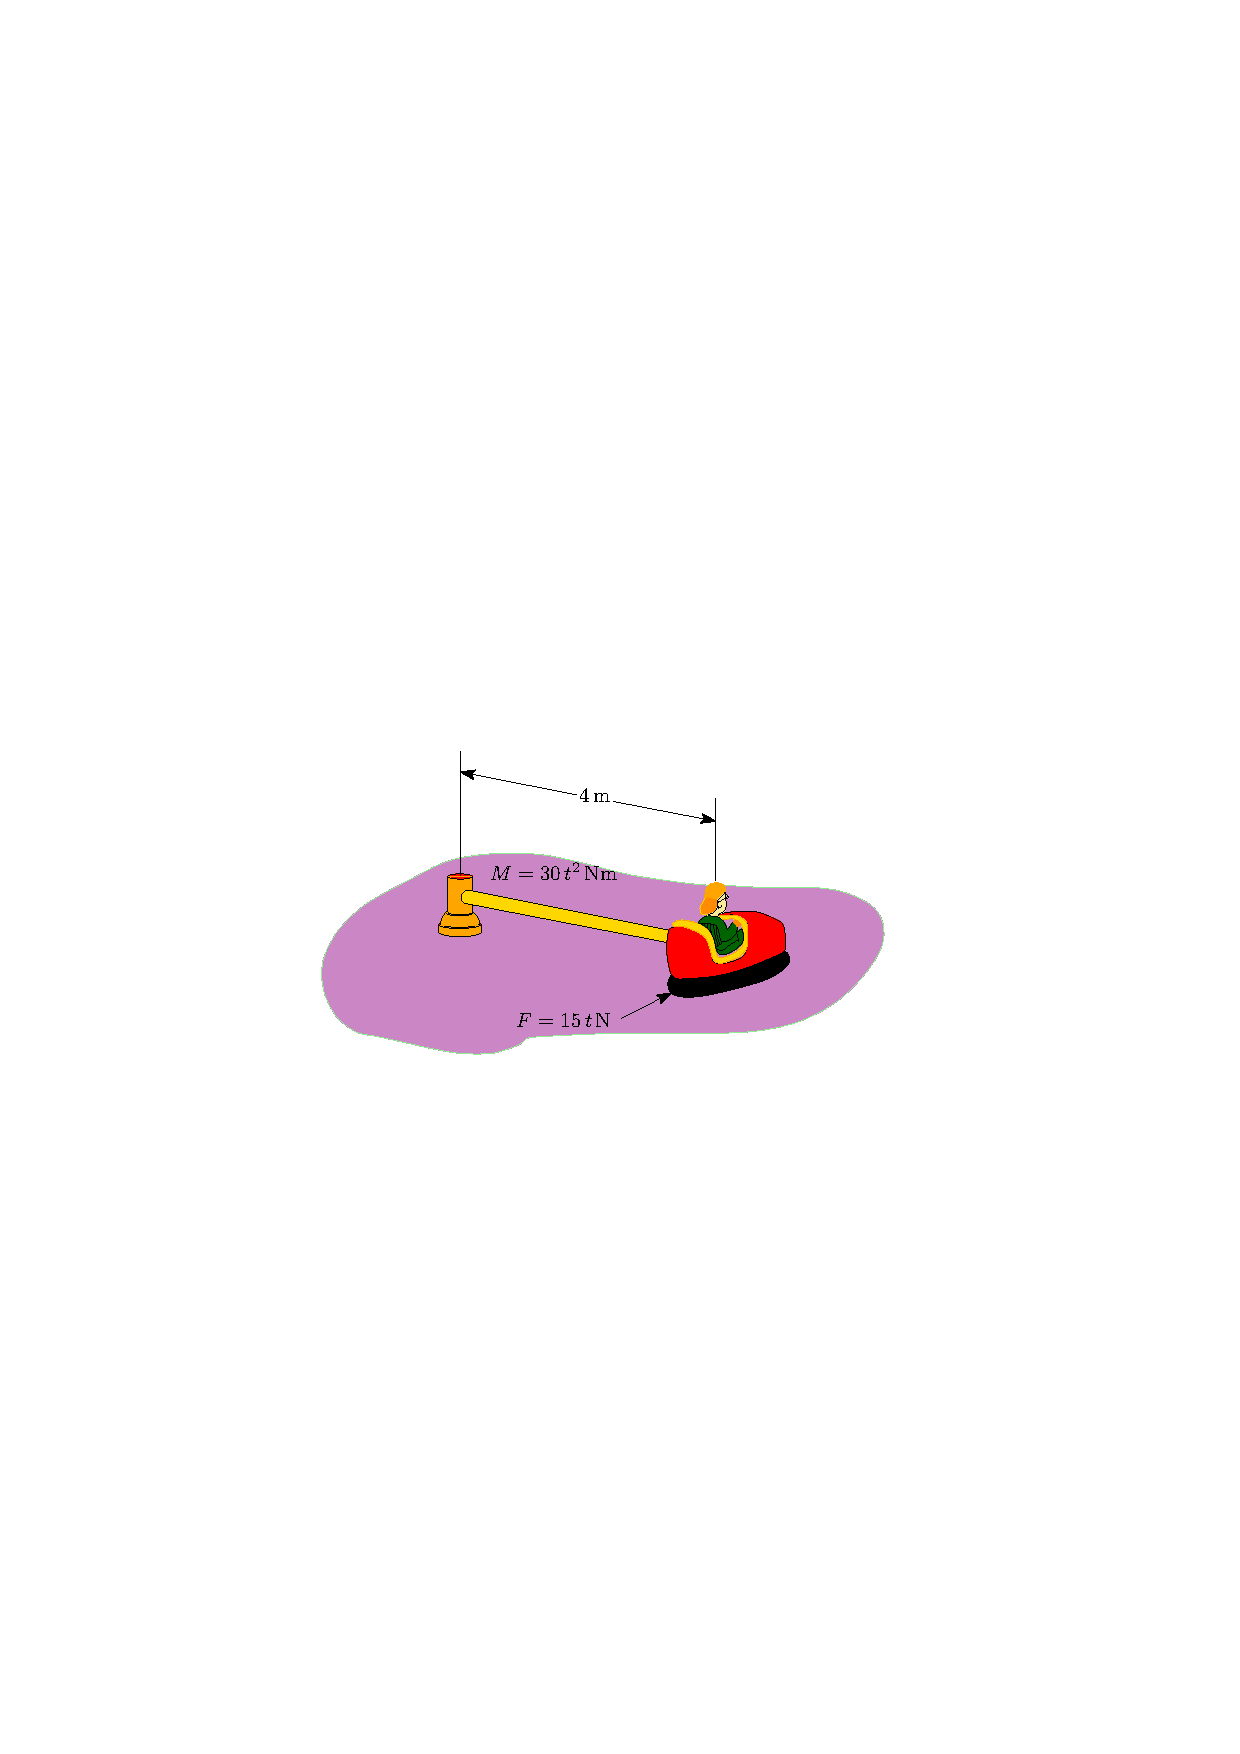
\includegraphics[scale=1.2]{images/draw_12}
\end{flushright}